\documentclass{beamer}

\usepackage{eurosym}
\usepackage{amsfonts}
\usepackage{amssymb}
\usepackage{amsmath}
%\usepackage{tipa}
\usepackage{array}
\usepackage{booktabs}
\usepackage{color}
\usepackage{epsfig,amssymb,latexsym,verbatim}
\usepackage{float}
\usepackage{graphicx}
\usepackage{graphicx, amssymb}
\graphicspath{{defense_ppt/}{./}}
\usepackage{hyperref}
\usepackage{multicol}
\usepackage{multirow}
\usepackage{subfigure}
\usepackage{framed}
\usepackage{pifont}
\usepackage{colortbl}
\usepackage{comment}
\usepackage{booktabs}
\usepackage{ctex}

\newtheorem{lem}{引理}
\newtheorem{deff}{Definition}
\newtheorem{thm}{定理}
\newtheorem{proposition}{命题}
\newtheorem{coro}{推论}

\setcounter{MaxMatrixCols}{10}

\mode<presentation>

\def\cmd#1{\texttt{\color{red}\footnotesize $\backslash$#1}}
\def\env#1{\texttt{\color{blue}\footnotesize #1}}
\definecolor{deepblue}{rgb}{0,0,0.5}
\definecolor{deepred}{rgb}{0.6,0,0}
\definecolor{deepgreen}{rgb}{0,0.5,0}
\definecolor{halfgray}{gray}{0.55}
\definecolor{tsinghuapurple}{RGB}{175,0,26}
\definecolor{glassgrey}{rgb}{220,220,220}

% Set Colours
\mode<presentation> {
\usetheme{Madrid}
%\usecolortheme{beaver}
\setbeamercolor{structure}{bg=tsinghuapurple,fg=tsinghuapurple}
}
\author{李思雨}
\institute[SU]
{
\textbf{指导老师}: 张园园 \medskip \\ 
苏州大学数学科学学院
}

\DeclareMathOperator*{\argmax}{argmax}
\DeclareMathOperator*{\argmin}{argmin}
\DeclareMathOperator*{\BIC}{BIC}
\DeclareMathOperator*{\MSE}{MSE}

\begin{document}
 
\title[误差分布]{基于累积分布函数的非平稳空间序列统计推断}
\titlegraphic{
\includegraphics[width=2cm]{suda.jpeg}}
\date{2026/5/20}


\begin{frame}
\titlepage
\end{frame}

\begin{frame}{目录}
\begin{itemize}
\item 研究动机与思路 \medskip
\item 估计方法\medskip
\item 主要理论结果\medskip
\item 模拟研究 \medskip
\item 实际数据分析 \medskip
\item 总结
\end{itemize}
\end{frame}

\section{研究动机与思路}
\begin{frame}{研究动机与思路}
\begin{itemize}
\item \textbf{问题:} 
\begin{itemize}
\item 现有空间统计方法多适用规则网格区域, 难以处理\textbf{不规则图像域}(如带空洞或复杂边界).
\item 传统误差分布推断方法通常假设数据独立, 不适用于空间相关的图像数据.
\end{itemize}
\item \textbf{研究思路}
\begin{itemize}
\item 将不规则图像域划分为三角形网格, 构造局部多项式样条基函数(\cite{lai2013bivariate}, \cite{huq2023}), 用三角剖分上的二元样条(Bivariate Spline over Triangulations, BST)方法解决复杂边界和非矩形域的问题.
\item 在考虑数据空间相关性的前提下, 研究误差分布估计的Oracle有效性.(\cite{wang2020simultaneous}, \cite{wang2022oracle})
\item 基于估计的误差分布函数构造同时置信带(SCB), 量化不确定性.
(\cite{wang2020simultaneous})
\end{itemize}
\end{itemize}
\end{frame}


\section{估计方法}
\begin{frame}{估计方法：模型}
\begin{itemize}
    \item 本文考虑如下空间序列模型：
        \begin{equation}\label{model:nonparbiregression}
            Y_{\mathbf{i}} = g(X_{\mathbf{i}})+Z_{\mathbf{i}}, \mathbf{i}\in \mathcal{I}_n,
        \end{equation}
其中, $g(x):\mathbb{R}^2 \rightarrow \mathbb{R}$ 是未知的确定性趋势函数,  误差项$\{Z_{\mathbf{i}},\mathbf{i}\in\mathbb{Z}^2\}$ 为严格平稳的零均值空间过程. 其概率密度函数为 $f(z)$，分布函数为 $F(z)=\int_{-\infty}^{z}f(u)du$.
    \item 总数据量：$n$.
    \item 本文将原始指标集 $\mathcal{I}_n=\left\{\mathbf{i}_1,\cdots,\mathbf{i}_n\right\}$ 划分为两个互不相交的子集 $\mathcal{I}_{n'}=\left\{\mathbf{i}_{T_n},\mathbf{i}_{2T_n}\cdots,\mathbf{i}_{n'T_n}\right\}$ 和 $ \mathcal{I}_{n''} = \mathcal{I}_{n}/\mathcal{I}_{n'}$, 其中 $T_{n}$是小于$n$的正整数, $n' = [n/T_{n}], n''=n-n'$.
\end{itemize}
\end{frame}

\begin{frame}{估计方法：BST}
\begin{block}{数据划分}
\begin{itemize}
    \item 在数据集$\mathcal{I}_{n'}$上估计函数$g(\cdot)$;
    \item 基于数据集$\mathcal{I}_{n''}$计算残差$\hat{Z}_{\mathbf{i}'}$.
\end{itemize}
\end{block}

空间趋势函数 $g(\boldsymbol{x})$ 可近似表示为如下基函数展开形式：
\[
  g(\boldsymbol{x})
   \approx \sum_{l\in\mathcal{L}} B_l(\boldsymbol{x})\,\gamma_l
  = \mathbf{B}^\top(\boldsymbol{x})\,\boldsymbol{\gamma},
\]
其中 $\boldsymbol{\gamma}^\top=(\gamma_l,\,l\in\mathcal{L})$ 为样条系数向量.

给定空间过程 $\{Y_{\mathbf{i}}\}$ 的观测值$\mathbf{Y}=(Y_{\mathbf{i}''},\,\mathbf{i}''\in\mathcal{I}_{n''})^\top$，  
考虑以下最小二乘估计量：
\begin{equation}
  \hat{g}(\cdot)
  = \underset{s(\cdot)\in \mathbb{S}_{d}^{r}(\triangle)}{\mathrm{argmin}}
  \sum_{\mathbf{i}''\in\mathcal{I}_{n''}}\!
  \bigl\{Y_{\mathbf{i}''}-s(\boldsymbol{x}_{\mathbf{i}''})\bigr\}^2,
\end{equation}
其中，$\mathbb{S}_{d}^{r}(\triangle)$ 表示在三角剖分 $\triangle$ 上定义的次数为 $d$、光滑阶数为 $r$ 的样条函数空间.
\end{frame}

\begin{frame}{估计方法：BST}
\begin{block}{约束条件}
\begin{align}\label{EQ:RBSTLS}
   \underset{\boldsymbol{\gamma}}{\mathrm{argmin}}\sum_{\mathbf{i}''\in \mathcal{I}_{n''}}
   \Bigl\{Y_{\mathbf{i}''}-\mathbf{B}^{\top}(\boldsymbol{x}_{\mathbf{i}''})\boldsymbol{\gamma}\Bigr\}^2
   \quad\text{s.t. } \mathbf{H}\boldsymbol{\gamma}=0.
\end{align}
\end{block}

对 $\mathbf{H}^\top$ 进行 QR 分解：
\[
\mathbf{H}^\top
= \mathbf{Q}\mathbf{R}
= \begin{pmatrix}\mathbf{Q}_1 & \mathbf{Q}_2\end{pmatrix}
  \begin{pmatrix}\mathbf{R}_1\\ \mathbf{0}\end{pmatrix},
\]
其中$\mathbf{Q}$ 为正交矩阵；$\mathbf{R}_1$ 为上三角矩阵.
\end{frame}

\begin{frame}{估计方法：BST}
\small
\begin{block}{无约束最小二乘问题}
令$\boldsymbol{\gamma} = \mathbf{Q}_2\boldsymbol{\theta}$，
\begin{align}\label{EQ:RRBSTLS}
    \underset{\boldsymbol{\theta}}{\mathrm{argmin}}\sum_{\mathbf{i}''\in \mathcal{I}_{n''}}
   \Bigl\{Y_{\mathbf{i}''}-\mathbf{B}^{\top}(\boldsymbol{x}_{\mathbf{i}''})\mathbf{Q}_2\boldsymbol{\theta}\Bigr\}^2,
\end{align}
可得
\[
\hat{\boldsymbol{\theta}}
= \bigl(\tilde{\mathbf{B}}^\top \tilde{\mathbf{B}}\bigr)^{-1}
  \tilde{\mathbf{B}}^\top \mathbf{Y},
\quad
\hat{\boldsymbol{\gamma}}
= \mathbf{Q}_2
  \bigl(\tilde{\mathbf{B}}^\top \tilde{\mathbf{B}}\bigr)^{-1}
  \tilde{\mathbf{B}}^\top \mathbf{Y},
\]
其中$\tilde{\mathbf{B}}=\mathbf{B}\mathbf{Q}_2.$
\end{block}

\begin{block}{BST 估计函数}
    \begin{align}\label{EQ:BSTghat}
  \hat{g}(\boldsymbol{x})
  = \mathbf{B}^\top(\boldsymbol{x})\,\hat{\boldsymbol{\gamma}}
  = \mathbf{P}(\boldsymbol{x})\,\mathbf{Y},
\end{align}
其中投影矩阵
\(
\mathbf{P}(\boldsymbol{x})
= \mathbf{B}^\top(\boldsymbol{x})\,\mathbf{Q}_2\,
  \bigl(\tilde{\mathbf{B}}^\top \tilde{\mathbf{B}} \bigr)^{-1}
  \tilde{\mathbf{B}}^\top.
\)

\end{block}
\end{frame}

\begin{frame}{估计方法：BST}
    将式 \eqref{EQ:BSTghat} 代入模型 \eqref{model:nonparbiregression}
可得分解：
\begin{align}\label{EQ:ghat}
  \hat{g}(\boldsymbol{x})
  = \tilde{g}(\boldsymbol{x}) + \tilde{Z}(\boldsymbol{x}),
\end{align}

其中，
\begin{align}\label{gtilde}
  \tilde{g}(\boldsymbol{x})
  &= \mathbf{B}^\top(\boldsymbol{x})\,\mathbf{Q}_2
     (\tilde{\mathbf{B}}^\top \tilde{\mathbf{B}})^{-1}
     \tilde{\mathbf{B}}^\top \mathbf{g},\\[0.3em]
\label{Ztilde}
  \tilde{Z}(\boldsymbol{x})
  &= \mathbf{B}^\top(\boldsymbol{x})\,\mathbf{Q}_2
     (\tilde{\mathbf{B}}^\top \tilde{\mathbf{B}})^{-1}
     \tilde{\mathbf{B}}^\top \mathbf{Z},
\end{align}
\[
\mathbf{g} = (g(\boldsymbol{x}_{\mathbf{i}''}), \mathbf{i}''\in \mathcal{I}_{n''})^\top,\quad
\mathbf{Z} = (Z_{\mathbf{i}''}, \mathbf{i}''\in \mathcal{I}_{n''})^\top.
\]
\end{frame}


\begin{frame}{估计方法：KDE}
\begin{block}{核分布估计量}
不可行核分布估计量：
\begin{equation}\label{EQ:Fn'tilde}
\tilde{F}_{n',h}(z)
= \int_{-\infty}^{z} \tilde{f}(u) \, du
= n'^{-1} \sum_{\mathbf{i}' \in \mathcal{I}_{n'}}
\int_{-\infty}^{z} K_h(u - Z_{\mathbf{i}'}) \, du, 
\quad z \in \mathbb{R},
\end{equation}
其中 $K$ 为核函数, $K_h(u) = h^{-1} K(u/h)$, $h>0$ 为带宽参数.
\end{block}
\begin{block}{光滑同时置信带(SCB)的构造}
基于$\tilde{F}_{n',h}(z)$可构造如下光滑同时置信带：
\begin{align} \label{SCB:Ftilden'}
    \left[ \tilde{F}_{n',h}(z) - \frac{L_{1-\alpha}}{\sqrt{n'}},\tilde{F}_{n',h}(z) + \frac{L_{1-\alpha}}{\sqrt{n'}} \right] \cap [0,1], \quad z \in \mathbb{R}.
\end{align}
\end{block}
\end{frame}

\begin{frame}{估计方法：KDE}
\begin{block}{核分布估计量}
oracle核分布估计量：
\begin{equation}\label{EQ:FN'hhat-copy}
    \hat{F}_{n',h}(z) = \int_{-\infty}^{z}\hat{f}(u)du = n'^{-1}\sum_{\mathbf{i}'\in\mathcal{I}_{n'}}\int_{-\infty}^z K_h(u-\hat{Z}_{\mathbf{i}'})du,z\in\mathbb{R},
\end{equation}
其中残差$\hat{Z}_{\mathbf{i}'} = Y_{\mathbf{i}'} - \hat{g}(x_\mathbf{i'})$ 用于逼近真实误差 $Z_{\mathbf{i}'} = Y_{\mathbf{i}'} - g(x_\mathbf{i'})$, $\mathbf{i}'\in\mathcal{I}_{n'}$. 
\end{block}
\begin{block}{光滑同时置信带(SCB)的构造}
基于$\hat{F}_{n',h}(z)$可构造如下光滑同时置信带：
\begin{align} \label{SCB:Fhatn'h}
    \left[\hat{F}_{n',h}(z)-\frac{L_{1-\alpha}}{\sqrt{n'}}, \hat{F}_{n',h}(z)+\frac{L_{1-\alpha}}{\sqrt{n'}}\right] \cap [0,1], z \in \mathbb{R},
\end{align}
\end{block}
\end{frame}

\begin{frame}{估计方法：KDE}
\begin{block}{经验边际分布函数}
作为对比, 本文同时考虑一种 ``非光滑'' 的经验边际分布函数 EMDF:
\begin{equation} \label{EQ:Fn'hat}
    \hat{F}_{n'}(z) = n'^{-1}\sum_{\mathbf{i}'\in\mathcal{I}_{n'}} I(\hat{Z}_{\mathbf{i}'} \le z), \quad z \in \mathbb{R}.
\end{equation}
\end{block}
\begin{block}{非光滑同时置信带}
将方程~(\ref{SCB:Fhatn'h}) 中的 $\hat{F}_{n',h}$ 替换为 $\hat{F}_{n'}$, 即可得到对应的 ``非光滑'' 同时置信带:
\begin{align} \label{SCB:Fhatn'}
    \left[ \hat{F}_{n'}(z) - \frac{L_{1-\alpha}}{\sqrt{n'}},  \hat{F}_{n'}(z) + \frac{L_{1-\alpha}}{\sqrt{n'}} \right] \cap [0,1], \quad z \in \mathbb{R},
\end{align}

\end{block}
\end{frame}

\begin{frame}{理论假设}
下面是本文用到的一些基础假设：

\begin{itemize}
\item[(A1)] 累积分布函数 $F(\cdot) \in \mathcal{C}^{(1,1)}(\mathbb{R})$, 其密度函数 $f(\cdot)$ 满足 $\Vert f \Vert_{\infty} \leq C_f$, 其中常数 $C_f > 0$.

\item[(A2)] 非平稳空间趋势函数 $g(\cdot) \in \mathcal{W}^{\ell+1, \infty}(\Omega)$, 其中 $\ell \geq 1$ 为整数.

\item[(A3)] 空间误差过程 $\{ Z_{\mathbf{i}} \}_{\mathbf{i} \in \mathcal{I}_n}$ 是严格平稳且满足 $\alpha$-混合条件, 并具有有限矩
\[
M_{2+\delta} = \mathrm{E}|Z|^{2+\delta} < \infty,
\]
其中 $\delta > 0$. 此外, 存在常数 $C_\rho > 0$ 和 $\rho \in (0,1)$, 使得
\[
\alpha(k; i, j) \leq C_\rho\, i\, \rho^k, \quad \text{对于所有 } i, j, k \geq 1,
\]
其中 $\alpha(k; i, j)$ 表示强混合系数, 且常数 $C_\rho$ 与 $\rho$ 与 $i, j, k$ 无关.
\end{itemize}
\end{frame}

\begin{frame}{理论假设}
\begin{itemize}
\item[(A4)] 剖分 $\triangle$ 是 $\pi$-准均匀的. 三角形数量满足 $N = |\triangle|^{-2} = C n^\theta$, 其中常数 $C > 0$, $\theta \in [1/(\ell+2),\,1)$. 相邻采样点之间的间距满足
\[
T_n \sim |\triangle|^{-2} (\log n)^a, \quad a > 0.
\]
\label{Assumption:Delta}

\item[(A5)] 核函数 $K \in \mathcal{C}^{(2,1)}(\mathbb{R})$ 是对称的概率密度函数, 其导函数 $K'$ 与 $K''$ 的支撑均为紧集, 且位于区间 $[-1,1]$ 内.

\item[(A6)] 带宽满足 $h = h_n = n'^{-t} c_n$, 其中 $c_n + c_n^{-1} = {\scriptstyle{\mathcal{O}}}(\log^\tau n)$ (对任意 $\tau > 0$), 且 $t \in [1/4, 1/3]$. 此外, 当 $t = 1/4$ 时有 $c_n \to 0$ (当 $n \to \infty$).
\end{itemize}
\end{frame}

\section{主要理论结果}
\begingroup
\setbeamertemplate{theorems}[numbered]
\setcounter{proposition}{0}
\begin{frame}
\footnotesize
\begin{coro}\label{colrollary:ftilde}
假设条件 (A1)及(A3)--(A6) 成立, 则有
\begin{align*}
    &\left\Vert \tilde{f} \right\Vert_{\infty} = \mathcal{O}_{a.s.}(1),\\
    &\sup_{z\in\mathbb{R}} n'^{-1}\sum_{\mathbf{i}'\in\mathcal{I}_{n'}}
    \left\vert K_h'(z-Z_{\mathbf{i}'}) \right\vert = \mathcal{O}_{a.s.}(1).
\end{align*}
\end{coro}

\begin{proposition}[\cite{Yao2003ExponentialIF},\cite{bosq2012nonparametric}]
    在假设(A1)-(A4)成立的前提下, 当$n\to\infty$时,
    \[
\left\lVert \tilde{g} - g \right\rVert_{\infty} = \sup_{\boldsymbol{x} \in \Omega} \left| \tilde{g}(\boldsymbol{x}) - g(\boldsymbol{x}) \right| = \mathcal{O}_{a.s.} \left( |\triangle|^{\ell+1} \right),
\]
\end{proposition}

\begin{proposition}
[\cite{lai2007spline},\cite{yu2019estimation}]
  在假设(A1)-(A4)成立的前提下, 当 $n\to\infty$时,
  \[
\left\lVert \tilde{Z} \right\rVert_{\infty} = \sup_{\boldsymbol{x} \in \Omega} \left| \tilde{Z}(\boldsymbol{x}) \right| = \mathcal{O}_p \left( n''^{-1/2} |\triangle|^{-1} (\log n)^{1/2} \right),
\]
\end{proposition}

\end{frame}

\begin{frame}
由命题 1 和命题 2 可推导出命题 3.

\begin{proposition}
    在假设(A1)-(A4)成立的前提下, 当 $n\to\infty$时,
   \[
\max_{\mathbf{i}' \in \mathcal{I}_{n'}} \left\lVert Z_{\mathbf{i}'} - \hat{Z}_{\mathbf{i}'} \right\rVert 
\le \left\lVert \hat{g} - g \right\rVert_{\infty}
= \mathcal{O}_p \left( |\triangle|^{\ell+1} + n''^{-1/2} |\triangle|^{-1} (\log n)^{1/2} \right).
\]
\end{proposition}
\end{frame}
\endgroup


\begin{frame}{定理\uppercase\expandafter{\romannumeral 1}}
\begin{thm} \label{THM:FhatFtilde}
在假设(A1)-(A6)成立的前提下, oracle估计量$\hat{F}_{n',h}(\cdot)$ 渐近等价于不可行估计量$\tilde{F}_{n',h}(\cdot)$, 即当$n\to\infty$时，
\begin{align*}
    D\left(\hat{F}_{n',h}, \tilde{F}_{n',h}\right) = \left\Vert\hat{F}_{n',h} - \tilde{F}_{n',h}\right\Vert_{\infty} = {\scriptstyle{\mathcal{O}}}_{p}\left(n'^{-1/2}\right).
\end{align*}
\end{thm}

\end{frame}

\begin{frame}{置信区间}

根据(\cite{fazekas2006asymptotic})的研究可知, 在指数衰减的混合条件以及足够稀疏的空间采样下，经验过程在分布意义下收敛到布朗桥:
\[
n'^{1/2}\left(F_{n'}(\cdot) - F(\cdot)\right) \overset{D}{\rightarrow} \mathcal{B}(F(\cdot)),
\]
其中$\mathcal{B}(\cdot)$ 是标准布朗桥.

结合上述定理\ref{THM:FhatFtilde}以及(\cite{wang2013smooth})的结果$\left\Vert \tilde{F}_{n',h} - F_{n'} \right\Vert_{\infty} = {\scriptstyle{\mathcal{O}}}_{p}\left(n'^{-1/2}\right),$ 
可得
$$\left\Vert \hat{F}_{n',h} - F_{n'} \right\Vert_{\infty} = {\scriptstyle{\mathcal{O}}}_{p}\left(n'^{-1/2}\right).$$
因此可推出如下结论：
\end{frame}


\begin{frame}{置信区间}
    \begin{coro}
  在假设(A1)-(A6)成立的前提下, 当 $n \to \infty$时,
    \[
\sqrt{n'}\left( \hat{F}_{n',h}(\cdot) - F(\cdot) \right) \overset{D}{\rightarrow} \mathcal{B}(F(\cdot)).
\]
特别地，由于对 \( \forall z \in \mathbb{R}\), \(\mathrm{E} \left\{ \mathcal{B}_{n'}(F(z)) \right\}^2 = F(z)\left\{1 - F(z)\right\},\)
所以我们可以得到
\[
n'^{1/2}\left\{ F(z)(1 - F(z)) \right\}^{-1/2} \left( \hat{F}_{n',h}(z) - F(z) \right) \overset{D}{\rightarrow}  N(0,1), \quad \forall z  \in \mathbb{R}.
\]
因此，当$\alpha \in (0,1)$时,
\begin{align*}
    \lim_{n \to \infty}P\left\{F(z) \in \hat{F}_{n',h}(z) \pm L_{1-\alpha}/\sqrt{n'}, z\in  \mathbb{R}\right\}=1-\alpha,
\end{align*}
 为$F(z)$的光滑同时置信带，(\ref{SCB:Fhatn'h})式是其定义式.
\end{coro}
\end{frame}


\section{模拟研究}
\begin{frame}{模拟研究}
\begin{itemize}
    \item 我们分别在规则矩形区域和不规则区域(shape)上计算了误差分布的估计量最大偏差.

    \item 数据生成的样本大小为\( (n_1, n_2) = (100, 50), (200, 100), (200, 200) \) 和 \( (500, 500) \).

    \item 数据由以下模型生成：
        $$Y_{\mathbf{i}} = g(x_1,x_2)+Z_{\mathbf{i}},\mathbf{1}\leq \mathbf{i}\leq \mathbf{n},$$
其中，回归函数为： $g(x_1,x_2) = sin(\pi x_1)+exp(-x_2^2)$.空间误差过程 \( Z_{i_1, i_2} \) 按如下空间移动平均(SMA)模型生成：
\[
Z_{i_1, i_2} = e_{i_1, i_2} + 0.3\, e_{i_1, i_2-1} + 0.3\, e_{i_1-1, i_2} + 0.1\, e_{i_1-1, i_2-1},
\]
其中 \( e_{i_1, i_2} \) 为来自标准正态分布 \( N(0,1) \) 的独立同分布误差项.
\end{itemize}
\end{frame}

\section{模拟研究}
\begin{frame}{模拟研究}
\begin{figure}[H]
    \centering 
    \setlength{\tabcolsep}{0pt} 
    \begin{tabular}{cc}
        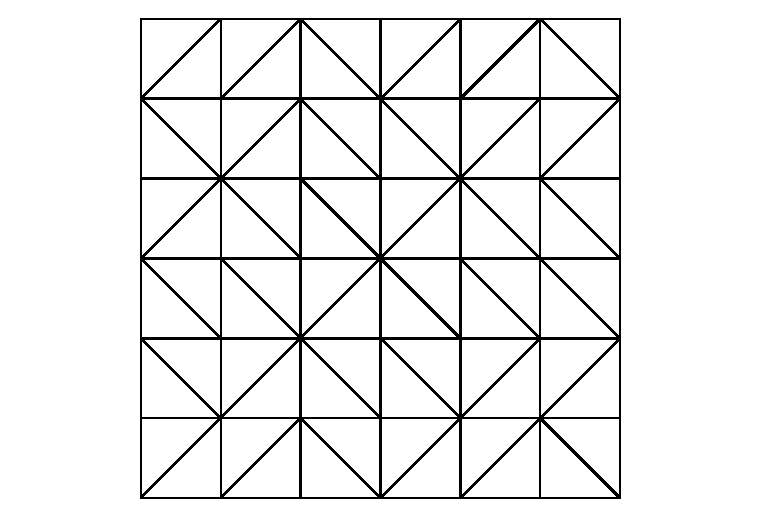
\includegraphics[width=0.5\textwidth]{tri_re6.pdf} &
        \hspace{-0.4in}
        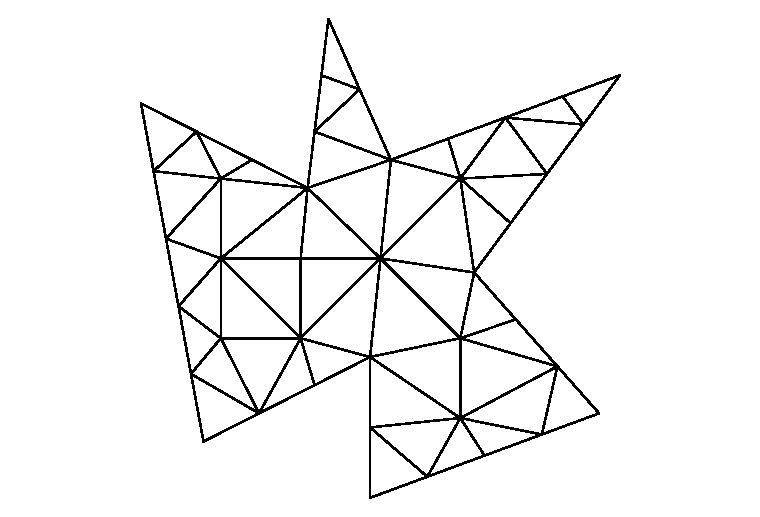
\includegraphics[width=0.5\textwidth]{tri_ir6.pdf} \\
        (a) & (b) \\
    \end{tabular}
    \caption{三角剖分示例：(a)矩形区域 (b) shape区域}
    \label{Fig:trigulation-sim}
\end{figure}

\end{frame}


\begin{frame}{模拟研究}
\small
\vspace{-0.3cm}
\begin{table}[!htb]
\caption{ 矩形区域和shape区域上三种估计量平均最大偏差的对比}
\begin{center}
\begin{tabular}{llcc}
        \toprule
        偏差 & $(n_1,n_2)$ & 规则区域 & shape区域 \\
        \midrule
        \multirow{4}{*}{$\bar{D}(\hat{F}_{n',h},F)$} 
            & $(100,50)$    & 0.0433 & 0.0571\\
            & $(200,100)$   & 0.0294 & 0.0300 \\
            & $(200,200)$   & 0.0209 & 0.0209 \\
            & $(500,500)$   & 0.0100 & 0.0144 \\
        \midrule
        \multirow{4}{*}{$\bar{D}(\hat{F}_{n'},F)$} 
            & $(100,50)$    & 0.0435 & 0.0577\\
            & $(200,100)$   & 0.0294 & 0.0302 \\
            & $(200,200)$   & 0.0225 & 0.0225 \\
            & $(500,500)$   & 0.0107 & 0.0153\\
        \midrule
        \multirow{4}{*}{$\bar{D}(\tilde{F}_{n',h},F)$} 
            & $(100,50)$    & 0.0425 & 0.0574 \\
            & $(200,100)$   & 0.0287 & 0.0292 \\
            & $(200,200)$   & 0.0199 & 0.0204 \\
            & $(500,500)$   & 0.0097 & 0.0140\\
        \bottomrule
    \end{tabular}
\end{center}
\end{table}
\end{frame}

\begin{frame}{模拟研究}
\vspace{-0.3cm}
\begin{table}[!htb]
\caption{ 矩形区域上同时置信带覆盖率的对比}
\begin{center}
\footnotesize 
\renewcommand{\arraystretch}{0.8} 
\begin{tabular}{lccccc}
\toprule
\multirow{2}{*}{$(n_1,n_2)$} & \multirow{2}{*}{$1-\alpha$} & \multicolumn{3}{c}{覆盖率} & \multirow{2}{*}{比较结果} \\ 
\cmidrule{3-5}
& & $\hat{F}_{n', h}$ & $\hat{F}_{n'}$ & $\tilde{F}_{n', h}$ & \\ 
\midrule
$(100,50)$  & 0.99 & 0.988 & 0.986 & 0.988 & $\ast$ \\
            & 0.95 & 0.936 & 0.932 & 0.954 & -- \\
            & 0.90 & 0.892 & 0.876 & 0.872 & $\ast\ast$ \\
            & 0.80 & 0.810 & 0.806 & 0.788 & $\ast\ast$ \\ \addlinespace
$(200,100)$ & 0.99 & 0.988 & 0.988 & 0.994 & $\ast\ast$ \\
            & 0.95 & 0.940 & 0.940 & 0.958 & -- \\
            & 0.90 & 0.890 & 0.892 & 0.910 & $\ast$ \\
            & 0.80 & 0.806 & 0.812 & 0.836 & $\ast\ast$ \\ \addlinespace
$(200,200)$ & 0.99 & 0.984 & 0.976 & 0.998 & $\ast\ast$ \\
            & 0.95 & 0.944 & 0.932 & 0.964 & $\ast\ast$ \\
            & 0.90 & 0.902 & 0.860 & 0.926 & $\ast\ast$ \\
            & 0.80 & 0.810 & 0.764 & 0.850 & $\ast\ast$ \\ \addlinespace
$(500,500)$ & 0.99 & 0.992 & 0.984 & 0.992 & $\ast$ \\
            & 0.95 & 0.954 & 0.936 & 0.968 & $\ast\ast$\\
            & 0.90 & 0.896 & 0.874 & 0.932 & $\ast\ast$ \\
            & 0.80 & 0.828 & 0.778 & 0.864 & $\ast\ast$\\ 
\bottomrule
\end{tabular}
\end{center}
\end{table}
\end{frame}

\begin{frame}{模拟研究}
\vspace{-0.1cm}
\begin{figure}
\vspace{-0.5cm}
\caption{矩形区域上$D\left( \hat{F}_{n^{\prime },h},F\right)$ 的箱线图 }
\centering
    \begin{minipage}[t]{\linewidth}
        \centering
        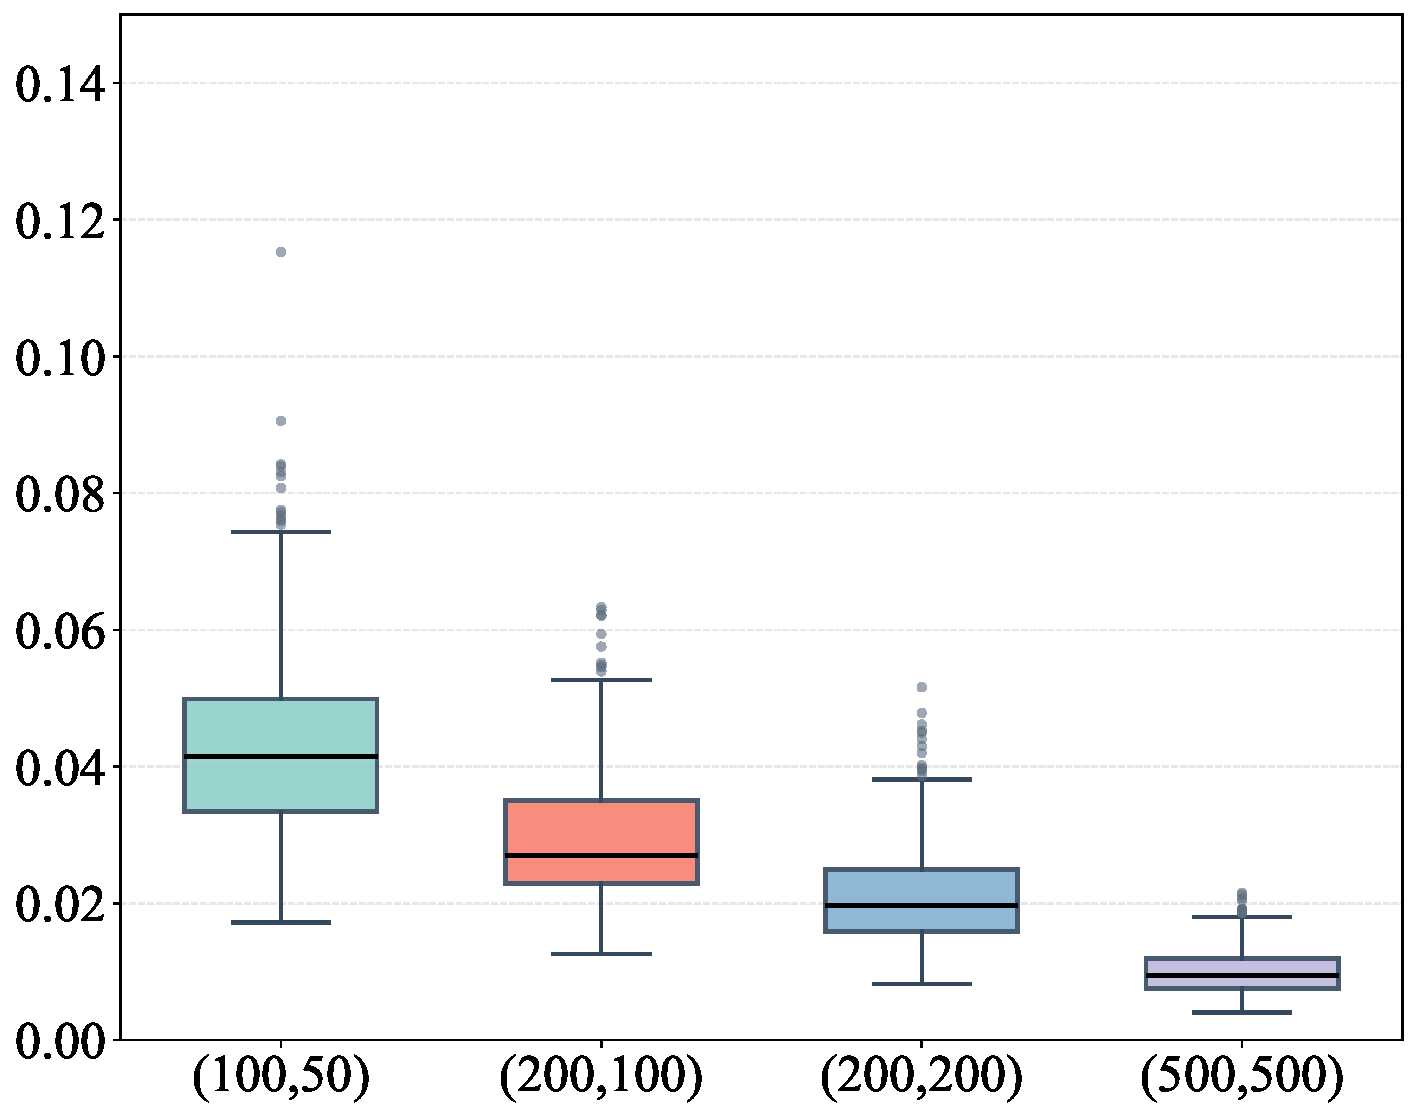
\includegraphics[width=0.7\linewidth]{bpNregular.pdf}
    \end{minipage}
\end{figure}
\end{frame}

\begin{frame}{模拟研究}
\vspace{-0.3cm}
\begin{table}[!htb]
\caption{ 不规则区域上同时置信带覆盖率的对比}
\begin{center}
\footnotesize 
\renewcommand{\arraystretch}{0.8} 
\begin{tabular}{lccccc}
\toprule
\multirow{2}{*}{$(n_1,n_2)$} & \multirow{2}{*}{$1-\alpha$} & \multicolumn{3}{c}{覆盖率} & \multirow{2}{*}{比较结果} \\ 
\cmidrule{3-5}
& & $\hat{F}_{n', h}$ & $\hat{F}_{n'}$ & $\tilde{F}_{n', h}$ & \\ 
\midrule
$(100,50)$  & 0.99 & 0.988 & 0.986 & 0.988 & $\ast$ \\
            & 0.95 & 0.966 & 0.966 & 0.960 &  -- \\
            & 0.90 & 0.916 & 0.910 & 0.914 &  -- \\
            & 0.80 & 0.818 & 0.814 & 0.860 & $\ast\ast$ \\ \addlinespace
$(200,100)$ & 0.99 & 0.998 & 0.998 & 0.996 & -- \\
            & 0.95 & 0.966 & 0.960 & 0.968 & -- \\
            & 0.90 & 0.914 & 0.910 & 0.912 & -- \\
            & 0.80 & 0.814 & 0.816 & 0.810 & $\ast\ast$ \\ \addlinespace
$(200,200)$ & 0.99 & 0.992 & 0.990 & 0.992 & $\ast$ \\
            & 0.95 & 0.960 & 0.956 & 0.974 & $\ast\ast$ \\
            & 0.90 & 0.914 & 0.892 & 0.930 & $\ast\ast$ \\
            & 0.80 & 0.828 & 0.798 & 0.838 & $\ast\ast$ \\ \addlinespace
$(500,500)$ & 0.99 & 0.988 & 0.986 & 0.996 & $\ast\ast$ \\
            & 0.95 & 0.954 & 0.940 & 0.962 & $\ast\ast$ \\
            & 0.90 & 0.906 & 0.888 & 0.910 & $\ast\ast$ \\
            & 0.80 & 0.814 & 0.770 & 0.834 & $\ast\ast$ \\ 
\bottomrule
\end{tabular}
\end{center}
\end{table}
\end{frame}

\begin{frame}{模拟研究}
\vspace{-0.1cm}
\begin{figure}
\vspace{-0.5cm}
\caption{ 不规则区域上$D\left( \hat{F}_{n^{\prime },h},F\right) $ 的箱线图}
\centering
        \begin{minipage}[t]{\linewidth}
        \centering
        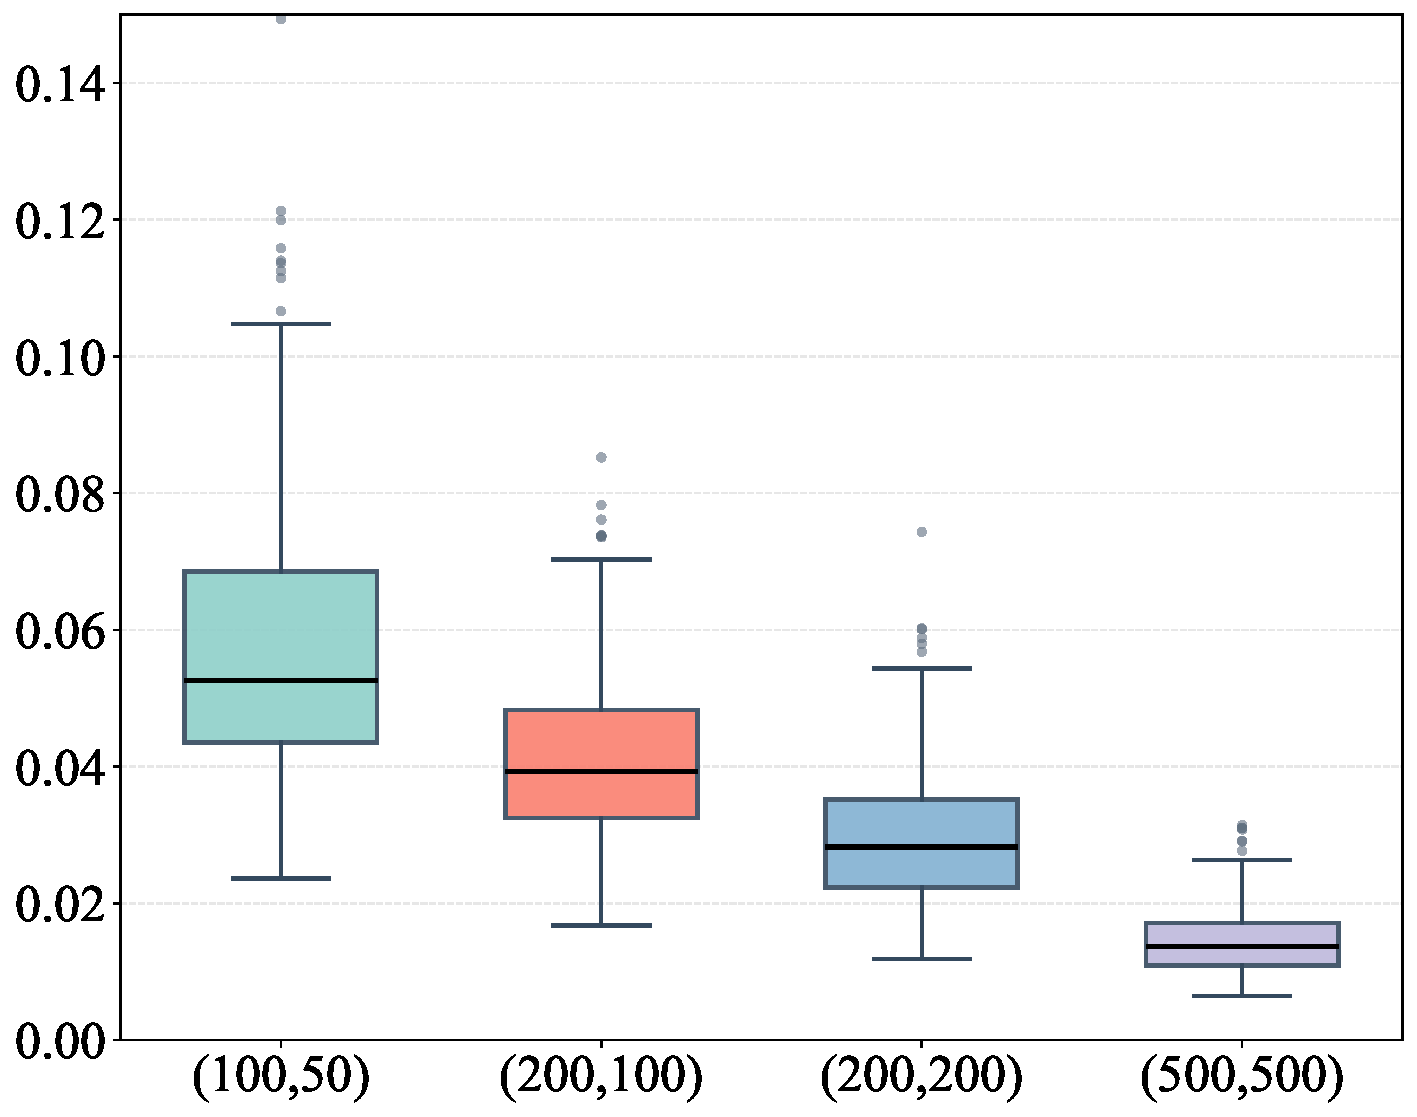
\includegraphics[width=0.7\linewidth]{bpNirregular.pdf}
    \end{minipage}
\end{figure}
\end{frame}

\section{实际数据分析}
\begin{frame}{实际数据分析}
\begin{itemize}
    \item 真实数据\uppercase\expandafter{\romannumeral 1}选取黑海海表温度数据. \cite{huq2023}, \cite{cai2024global}.
        \begin{itemize}
            \item 黑海经纬度范围：$40.5^{\circ}$N - $47.6^{\circ}$N和$26.8^{\circ}$E - $42.2^{\circ}$E.
            \item 数据来源：
    \url{https://marine.copernicus.eu}.
        \end{itemize}
    \item 真实数据\uppercase\expandafter{\romannumeral 2}选取全球大气二氧化碳浓度数据.
         \begin{itemize}
            \item 数据格点为$2.5^{\circ}\times 2^{\circ}$.
            \item 数据来源：\url{http://www.geodoi.ac.cn}.
        \end{itemize}
       
\end{itemize}
\end{frame}

\begin{frame}{实际数据}
\vspace{-0.1cm}
\begin{figure}
\vspace{-0.5cm}
\caption{黑海海表温度数据}
\centering
    \begin{minipage}[t]{\linewidth}
        \centering
        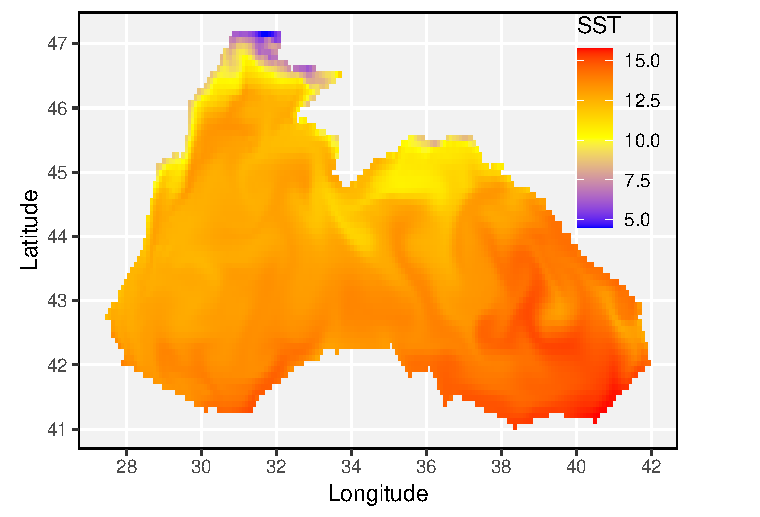
\includegraphics[width=0.7\linewidth]{heatmap09.pdf}
    \end{minipage}
\end{figure}
\end{frame}

\begin{frame}{实际数据}
\vspace{-0.1cm}
\begin{figure}
\vspace{-0.5cm}
\caption{全球大气二氧化碳浓度数据}
\centering
    \begin{minipage}[t]{\linewidth}
        \centering
        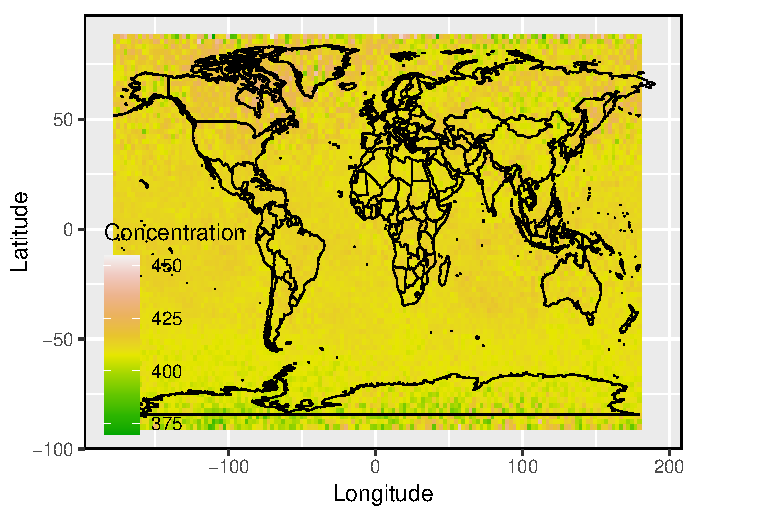
\includegraphics[width=0.7\linewidth]{Y_CO2.pdf}
    \end{minipage}
\end{figure}
\end{frame}

\section{总结}
\begin{frame}{总结}
\begin{itemize}
    \item 在假设(A1)-(A6)成立的前提下，证明了二维区域上非平稳空间序列误差分布估计的渐近理论, oracle效率为${\scriptstyle{\mathcal{O}}}_{p}\left(n'^{-1/2}\right)$.
    \item 构建了适用于复杂区域的误差分布同时置信带(SCB).
\end{itemize}
\end{frame}


\begin{frame}[allowframebreaks]{References}
\tiny
\begin{thebibliography}{20}

\bibitem[Hu(2023+)]{huq2023}
Hu Qirui and Li Jie (2023+). Statistical inference for mean function of longitudinal imaging data over complicated domains. Statistica Sinica 34, 955-982.
\bibitem[Cai(2024)]{cai2024global}
Cai, Leheng and Hu, Qirui (2024). Global inference and test for eigensystems of imaging data over complicated domains. Journal of Computational and Graphical Statistics, 1-17.
\bibitem[Wang(2022)]{wang2022oracle}
Wang, Jiangyan and Gu, Lijie and Yang, Lijian (2022). Oracle-efficient estimation for functional data error distribution with simultaneous confidence band. Computational Statistics \& Data Analysi 167, 107363.
\bibitem[Lai(2013)]{lai2013bivariate}
Lai, Ming-Jun and Wang, Li (2013). Bivariate penalized splines for regression. Statistica Sinica 23, 1399-1417.
\bibitem[Wang(2020)]{wang2020simultaneous}
Wang, Yueying and Wang, Guannan and Wang, Li and Ogden, R Todd (2020). Simultaneous confidence corridors for mean functions in functional data analysis of imaging data. Biometrics 76(2), 427-437.
\bibitem[Lai(2007)]{lai2007spline}
Lai, Ming-Jun and Schumaker, Larry L (2007). Spline Functions on Triangulations. Cambridge University Press.
\bibitem[Yu(2019)]{yu2019estimation}
Yu, Shan and Wang, Guannan and Wang, Li and Liu, Chenhui and Yang, Lijian (2019). Estimation and inference for generalized geoadditive models. Journal of the American Statistical Association 115, 761-774.
\bibitem[Bosq(2012)]{bosq2012nonparametric}
Bosq, Denis (2012). Nonparametric Statistics for Stochastic Processes: Estimation and Prediction. Springer Science \& Business Media.
\bibitem[Yao(2003)]{Yao2003ExponentialIF}
Yao, Qiwei (2003). Exponential inequalities for spatial processes and uniform convergence rates for density estimation. Development Of Modern Statistics And Related Topics, 118-128.
\bibitem[Fazekas(2006)]{fazekas2006asymptotic}
Fazekas, Istv{\'a}n and Chuprunov, Alexey (2006). Asymptotic normality of kernel type density estimators for random fields. Statistical inference for stochastic processes 9, 161-178.
\bibitem[Wang(2013)]{wang2013smooth}
Wang, Jiangyan and Cheng, Fuxia and Yang, Lijian (2013). Smooth simultaneous confidence bands for cumulative distribution functions. Journal of Nonparametric Statistics, 395-407.
\end{thebibliography}
\end{frame}

\begin{frame}
\begin{center}
\Huge{ 谢谢大家 !}
\end{center}
\end{frame}

\end{document}
